\documentclass[11pt,letter,twoside]{mc2011}
\usepackage{amsmath}
\usepackage{array}
%\usepackage{color}
\usepackage{graphicx}
\usepackage{float} %utiliser H pour forcer � mettre l'image o� on veut
\usepackage{lscape} %utilisation du mode paysage
\usepackage{mathbbol} % permet d'avoir le vrai symbol pour les reels grace a mathbb
\usepackage{enumerate}
\usepackage{marvosym}	
\usepackage{moreverb} % permet d'utiliser verbatimtab : conservation la tabulation 
\usepackage{lineno}


\setlength {\textwidth}{16cm}
\setlength {\textheight}{21cm} 
\setlength {\oddsidemargin}{0cm}
\setlength{\headsep}{5pt} 

\newcommand\bn{\boldsymbol{\nabla}}
\newcommand\bo{\boldsymbol{\Omega}}
\newcommand\br{\mathbf{r}}
\newcommand\la{\left\langle}
\newcommand\ra{\right\rangle}
\newcommand\bs{\boldsymbol}
\newcommand\red{\textcolor{red}}

\renewcommand{\(}{\left(}
\renewcommand{\)}{\right)}
\renewcommand{\[}{\left[}
\renewcommand{\]}{\right]}

\newtheorem{theorem}{Theorem}[section]

\usepackage[numbers,sort&compress]{natbib}

\usepackage{fancyhdr,lastpage}

%\usepackage[dvips]{graphicx,color}

\pagestyle{fancy}

\globalmc2011

\begin{document}
%\linenumbers
\title{To reduce memory needs for coupled photon-electron transport.}
\author{
    \textbf{Bruno Turcksin, Jean Ragusa, and Jim Morel}\\
    Texas A\&M University, Department of Nuclear Engineering\\
    College Sation, Texas 77843-3133\\
    turcksin@neo.tamu.edu; ragusa@ne.tamu.edu; morel@ne.tamu.edu
}
\date{}
\maketitle

\thispagestyle{empty}

% Abstract
\begin{abstract}
In this work, we present two methods to decrease memory needs while solving 
the photon-electron transport equation. The coupled transport of electrons and
photons is of importance in radiotherapy because it describes the interactions of
X-rays with matter. One of the issues of discretized electron transport is that the
electron scattering is very forward peaked. A common approximation is to
represent the peak in the scattering cross section by a Dirac distribution.
This is convenient, but the integration over all angles of this distribution requires the
use of Galerkin quadratures. By construction these quadratures impose that
the number of flux moments be equal to the number of directions 
(number of angular fluxes), which is very demanding in terms of memory. In this study, 
we show that even if the number of moments is not as large as the number 
of directions, an accurate solution can be obtained when using Galerkin
quadratures. Another method to decrease the 
memory needs involves choosing an appropriate reordering of the energy
groups. 
We show in this paper that an appropriate alternation of photons/electrons groups 
allows us to rewrite one transport problem of $n$ groups as $gcd$ successive 
transport problems of $\frac{n}{gcd}$ groups where $gcd$ is the greatest common 
divisor between the number of photon groups and the number of electron groups.
\keywords{Galerkin quadrature, photon-electron transport, radiotherapy}
\end{abstract}


\newcommand\authorname{Bruno Turcksin, Jean Ragusa, and Jim Morel}
\newcommand\shorttitlename{Methods to reduce memory needs for photon-electron transport.}

\fancymc2011

% Introduction
\section{Introduction}
The transport of photon and electron has a lot of applications in medical
physics and particularly in radiotherapy. The radiotherapy consists in sending
X-rays on a cancerous tumor in order to destroy it. The photons interact in the
body producing electrons by photo-electric effect. These electrons destroy the
cells but produce secondary photons which will also produce electron. One
quantity used to know if a cell will die or not is the absorbed dose. The
absorbed dose is defined as the energy deposition by unit of mass. The unit of the 
absorbed dose is the Gray ($GY=\frac{J}{kg}$). It is important to know accurately what
is the dose sent. The dose has to be large enough in the tumor to kill the
cancerous but as small as possible in the healthy cells. To compute this dose,
several methods can be applied :
\begin{description}
\item[Semi-analytic methods,] very fast but inaccurate.
\item[Deterministic method,] fast and accurate but needs a lot of memory.
\item[Monte-Carlo,] very accurate but slow to converge.
\end{description}
The goal of the radiotherapy is to sent a dose as high as possible while
sparing the healthy cells. It is very important to spare the healthy cells
because the radiation can cause cancer several years later. Thus, it is more
and more important to know the dose accurately. Monte-Carlo method are of
course a very interesting method to have very accurate results however they
are slow to converge. Nowadays, they remain too slow for effective clinical
use \cite{acuros}. Others methods are pencil-beam convolution and
convolution superposition employ the use of pre-calculated Monte-Carlo dose
kernels, which are then locally scaled to approximate photon and electron
transport in the presence of heterogeneities. These methods, however, have
some troubles in the presence of large density gradients, such as those at
interfaces between different materials : air, bone, lung and soft tissue 
\cite{acuros}. That is because of all the previous reasons that the
deterministic methods appear to be more and more interesting for radiotherapy. 
It has been shown in the past  that a very good agreement can be obtained
between deterministic method and Monte-Carlo method \cite{acuros}.\\
In this work, we will present a $S_n$ method for the photon-electron
transport. The difficulty of this calculation comes from the transport of the
electrons. The electrons are charged particles and thus, they have very
anisotropic scattering. This is due to the fact that can interact with others
particles through Coulomb interaction. Thus, the electrons have a lot of
interactions where the energy and the direction almost do not change. This 
anisotropy creates some problems since the standard Legendre expansion to represent 
the cross-sections would require hundreds of terms. A common approximation is to 
replace the Boltzmann equation by the Boltzmann-Fokker-Planck equation. These 
equation consists in adding in 2 terms: one causes to particles to redistribute in 
direction without energy change and the other to redistribute in energy without 
directional change\cite{morel_81}. This allows to keep the Legendre expansion of the 
cross-section to a low order. It is worth to note that the Henyey-Greenstein kernel
used to describe the scattering of light in biological tissues cannot be
expressed using the BFP equation \cite{larsen}. However, this model, even if
it is useful, because of its simplicity, has no theoretical root. The reason
is that the BFP equation assume that the scattering cross section is very
peaked. The Henyey-Greenstein is not peaked enough to be represented by the
BFP equation. We will see that it is very convenient to rewrite the term changing 
the direction as a Dirac distribution. However, an exact integration requires then to use the Galerkin quadrature \cite{graal}, which requires a lot of memory. 
Effectively, this quadrature needs that the number of flux moments and the
number of angular fluxes are equal. This number rises very quickly with the
order the $S_n$ method. For example, when using the $S_n$ discretization for $n=16$, 
we have, in 3D, 288 directions and thus, 288 angular fluxes or flux moments to
store. In this work, we will see the effects of truncation on the Galerkin
quadrature. The goal is to keep as few flux moments as possible while still
keeping an accurate solution.


% Equations
\section{Equations}                                                      
In this section, we present the equation that models the transport of
electrons. We will also show why it is so important to use Galerkin
quadratures. First, we present the 
Boltzmann-Fokker-Planck equation (BFP). The idea is to decompose the highly forward
peaked scattering cross section into a sum of a forward-peaked cross section
and a smoothly varying cross section. The BFP equation is given by (the variables are
omitted for brevity) \cite{morel_96} :
\begin{equation}
\begin{split}
\bo \cdot \bn \Psi + \Sigma_{t} \Psi &= \int_{4\pi}\int_0^{\infty} \Sigma_{s}\(\bo
\cdot \bo',E'\rightarrow E\) \Psi(\bo',E')dE'd\bo'\\
& + \frac{\alpha}{2}
\(\frac{\partial}{\partial \mu} \(1-\mu^2\) \frac{\partial \Psi}{\partial \mu}
+ \frac{1}{1-\mu^2} \frac{\partial^2 \Psi}{\partial \phi^2}\) +
\frac{\partial S\Psi}{\partial E}  + Q
\end{split}
\label{bfp}
\end{equation}
where : 
\begin{itemize}
\item $\Psi$ is the angular flux 
\item $\Sigma_t$ is the smooth-component of the total macroscopic cross section
\item $\Sigma_s$ is the smooth-component of the macroscopic differential scattering cross section
\item Q is a volumetric source
\item $\mu$ is the cosine of the directional polar angle
\item $\phi$ is the directional azimuthal angle
\end{itemize} 
The second and the third term of the 
right-hand-side change the direction of the particles without changing their energy 
and the fourth term changes the energy of the particles without changing their 
direction (continuous slowing-down term) \cite{morel_81}. The continuous slowing 
down is used for the ``soft" interactions that result in small-energy losses. The 
catastrophic interactions that result in large energy losses are represented with 
the standard Boltzmann operator. $\alpha$ is the restricted momentum transfer :
\begin{equation}
\alpha(E) = 2 \pi \int_0^E \int_{-1}^1 \Sigma_{ss}(E\rightarrow E',\mu_0) (1-\mu_0) 
d\mu_0 dE
\end{equation}
with $\mu_0 = \mu'\mu+\sqrt{\(1-\mu'^2\)\(1-\mu^2\)} cos\(\phi'-\phi\)$ and
$\Sigma_{ss}(E\rightarrow E', \mu_0)$ denotes the forward-peaked scattering
cross section.\\
$S$ is the restricted stopping power :
\begin{equation}
S(E) = 2\pi \int_0^{E} \int_{-1}^{1} \Sigma_{ss}(E\rightarrow E',\mu_0) \(E-E'\)d\mu_0 dE'
\end{equation}
The restricted stopping power is defined as the portion of the total stopping
power that is not due to catastrophic collisions.\\
Standard boundary conditions can be applied to (\ref{bfp}), the
most likely being the vacuum boundary conditions :
\begin{equation}
\Psi(\br,\bo,E) = 0 \ \ \ \textrm{ for } \bo \cdot \bs{n} < 0 \textrm{ and } \br
\in \partial \mathcal{D}_v
\end{equation}
and the incoming flux boundary conditions :
\begin{equation}
\Psi(\br,\bo,E) = g(\br,\bo,E)  \ \ \ \textrm{ for } \bo \cdot \bs{n} < 0 \textrm{ and } \br
\in \partial \mathcal{D}_i
\end{equation}
where $\partial \mathcal{D}_v$ is the boundary of the domain where vacuum
conditions are applied and $\partial \mathcal{D}_i$ is the boundary of the
domain where incoming flux conditions are applied.\\
In this work, we will use another approach and
retain only the asymptotic limit on the energy dependence but not the angular
dependence. We will keep the continuous slowing-down term and approximate the
forward peaked angular dependence by a Dirac distribution. The equation can be written as : 
\begin{equation}
\bo \cdot \bn \Psi + \Sigma_{t} \Psi = \int_{4\pi}\int_0^{\infty}
\Sigma_{s}\(\bo
\cdot \bo',E'\rightarrow E\) \Psi(\bo',E')dE'd\bo' + \int_{-1}^1 c
\delta(\mu-1) \Psi d\mu + \frac{\partial S\Psi}{\partial E} + Q
\label{solved}
\end{equation}
The continuous slowing-down term in the 
equation (\ref{solved}) can be either treated explicitly or it can be treated in 
the cross sections. The latter was done in the CEPXS
code which produces cross sections for photons and electrons transport \cite{cepxs}. 
In this work, we use cross sections produced by CEPXS to compute the coupled 
photon-electron transport. Unlike \cite{acuros}, we do not assume that the electrons 
do not produce photons. The system is fully coupled, meaning that photons produce 
electrons and electrons produce photons. Thus, there are some upscattering 
terms present in the scattering matrix even if there is not upscattering
physically. The upscattering is between particle types; a given particle can
only loses energy and creates others particle types which are represented by
the upscattering terms.\\
Next, we focus on the scattering term, assuming that this quantity has been
integrated over the energy \hbox{range :}
\begin{equation}
R = \int_{4\pi} \Sigma_{s} \(\bo \cdot \bo'\) \Psi\(\bo'\) d\bo' + \int_{-1}^1
c\delta (\mu-1) \Psi d\mu
\label{scattering}
\end{equation}
In a $S_n$ code, it is usual to write the discretized scattering source 
(\ref{scattering}) as a product of 3 \hbox{matrices \cite{graal} :}
\begin{equation}
\bs{R} = M \Sigma D \bs{\Psi}
\end{equation}
where $\bs{R}$ is the vector containing the scattering source, $\bs{\Psi}$ is
the vector containing all the flux moments, $D$ is the discrete-to-moment matrix 
which maps a vector of discrete angular flux values to a corresponding vector of flux
moments, $\Sigma$ is the scattering matrix which contains the moments of the 
scattering cross sections on its diagonal, and $M$ is the moment-to-discrete matrix 
which maps a vector of flux moments to a corresponding vector of discrete angular 
flux values. The Galerkin quadratures require that :
\begin{equation}
D = M^{-1}
\end{equation}
and, therefore, $M$ and $D$ have to be square matrices. This implies that the number of
moments is equal to the number of directions.\\
Galerkin quadratures integrate exactly a delta
function scattering and that is why we need to use them. To see this, assume that :
\begin{equation}
\Sigma(\mu) = \delta(\mu-1)
\end{equation}
It is obvious that :
\begin{equation}
\begin{split}
R &= \int_{-1}^1 \delta(\mu-1) \Psi(\mu) d\mu\\
&= \Psi
\end{split}
\end{equation}
Because $P_l(1)=1$ for all $l$, all of the Legendre expansion coefficients, $\Sigma_l$, for the 
delta function equal to unity and the cross-section matrix is the identity
matrix. We get :
\begin{equation}
\bs{R} = MD\bs{\Psi}= \bs{\Psi}
\end{equation}



% Memory
\section{Memory issue}
In the previous section, we showed that we must use a Galerkin quadrature to solve
(\ref{solved}) correctly. This may be a significant issue in terms of memory
requirements.  
For neutron transport, the scattering is less anisotropic than for electron
transport, and therefore, fewer flux moments than angular 
fluxes are needed. This is the reason why the information is stored as flux moments. 
However, Galerkin quadratures require the number of moments 
to be equal to the number of directions. This requirement is very restrictive and it 
is important to explore whether it is possible to decrease the number of moments 
while keeping a larger number of directions. In \cite{mem}, the authors used a 
Legendre expansion of the scattering cross section lower than that required by the 
Galerkin quadrature. They have shown a good agreement between their results 
and Monte-Carlo simulations. In the next section, we will study the effects of changing 
the order of the Legendre expansion while keeping a larger number of angular 
fluxes than the order of the scattering expansion. We proceed  by building 
the matrices $M$ and $D$ using the Galerkin quadrature, then truncate them 
to keep only a few moments. Therefore, $M$ and $D$ will be rectangular instead 
of square matrices. We show the results for two materials (Al and Au) 
and for different Legendre expansions.


% Results
\section{Results}
In this section we will show the results that we obtainfor the three materials
and we will compare them with ONELDANT\cite{cepxs}. ONELDANT is a code which
solve the BFP equation in one dimension using the cross sections generated by
CEPXS. The code that we are developing is three dimensional. To compare the 
results produced by the two codes, we use the same spatial discretization 
(linear discontinuous finite element) and equivalent angular discretization 
(Gauss-Legendre for ONELDANT and Gauss-Legendre-Chebyshev for our code). 
The number of cells is the same in the direction of comparison. The only 
difference is in the output. ONELDANT gives only the average dose on a cell and 
that our code give the value at a given point. To compare the value of the dose 
at a given point, we will interpolate the value given by ONELDANT.

\subsection{Water}
For this example, we are using a $S_{12}$ Galerkin-Legendre-Chebyshev
quadrature. The medium is 5 cm thick and there is an incoming flux of
photons. The direction of the flux is chosen to be the most normal direction
of the quadrature and the value of the flux is 1 $\frac{n}{cm^2s}$. The source 
of photons has an energy of 20 MeV and we use a cut-off energy of 0.01 MeV. 
Every particle that has an energy lower than 0.01 MeV is assumed to depose 
all its energy without moving further.\\
In the next table, we show the dose computed every centimeter using a
different scattering \hbox{order :}
\begin{table}[H]
\begin{center}
\caption{Dose in $\frac{MeV}{g}$ for different scattering orders}
\begin{tabular}{|c|c|c|c|c|c|c|}
\hline
Position & ONELDANT & order = 13 & order = 11 & order = 9 & order = 7 & order = 5 \\
\hline
0 & 4.92645e-3 &  &  &  &  &  \\
1 & 5.68274e-2 &  &  &  &  &  \\
2 & 1.05076e-1 &  &  &  &  &  \\
3 & 1.47528e-1 &  &  &  &  &  \\
4 & 1.82864e-1 &  &  &  &  &  \\
5 & 1.85907e-1 &  &  &  &  &  \\
\hline
\end{tabular}
\end{center}
\end{table}     

\subsection{Aluminium}
The setup of this problem, is the same as that of the previous one but the medium is
composed of aluminium. In the following table, we show the dose computed every 
centimeter using a different scattering order :
\begin{table}[H]
\begin{center}
\caption{Dose in $\frac{MeV}{g}$ for different scattering orders}
\begin{tabular}{|c|c|c|c|c|c|c|}
\hline
Position & ONELDANT & order = 13 & order = 11 & order = 9 & order = 7 & order = 5 \\
\hline
0 & 0.015003 & 0.0146404 & 0.0146402 & 0.0141156 & 0.0166718 & 0.0087276 \\
1 & 0.169908 & 0.1697907 & 0.1697890 & 0.1698012 & 0.1695422 & 0.1728969 \\
2 & 0.275425 & 0.2752749 & 0.2752729 & 0.2753298 & 0.2742052 & 0.2775113 \\
3 & 0.316307 & 0.3161310 & 0.3161307 & 0.3165279 & 0.3145572 & 0.3199176 \\
4 & 0.312283 & 0.3120572 & 0.3120566 & 0.3125514 & 0.3104412 & 0.3153226 \\
5 & 0.233048 & 0.2087631 & 0.2087634 & 0.2094064 & 0.2061794 & 0.2154810 \\
\hline
\end{tabular}
\end{center}
\end{table}     
The agreement between ONELDANT and our code using the full order is excellent.
The differences on the border of the domain are larger due to the fact that
the dose varies quickly and thus, the interpolation used to find the value at
a given point by ONELDANT is not very accurate.\\ 
We can see that if we except the border of the domain, the results obtained by
using a $P_5$ order for the scattering are very close to the results using the
full order. The reason is that the high order moments are very small. Below,
we show several moments, for different groups. The abscissa is the distance in
centimeter and the ordinate is the value of the flux in $\frac{particle}{cm^2
s}$.
\begin{figure}[H]
\begin{minipage}[b]{0.45\linewidth}
\centering
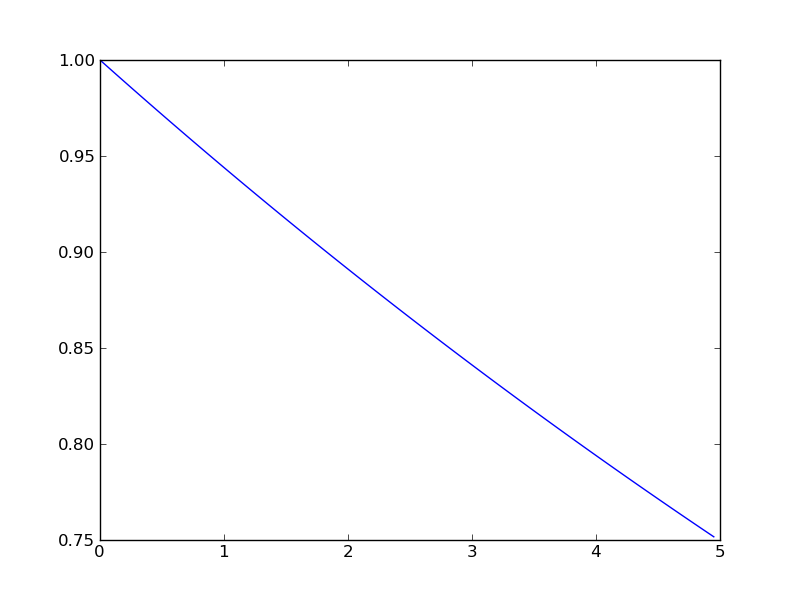
\includegraphics[width=\linewidth]{./images/al/group_0_moment_0}
\caption{Scalar flux for the first group of photons}
\end{minipage}
\hspace{0.5cm}
\begin{minipage}[b]{0.45\linewidth}
\centering
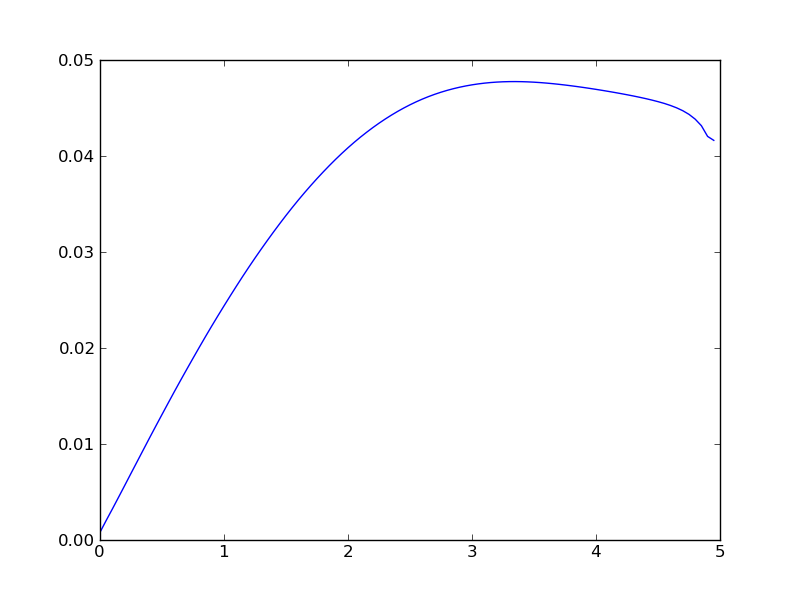
\includegraphics[width=\linewidth]{./images/al/group_39_moment_0}
\caption{Scalar flux for the last group of electrons}
\end{minipage}
\end{figure}

\begin{figure}[H]
\begin{minipage}[b]{0.45\linewidth}
\centering
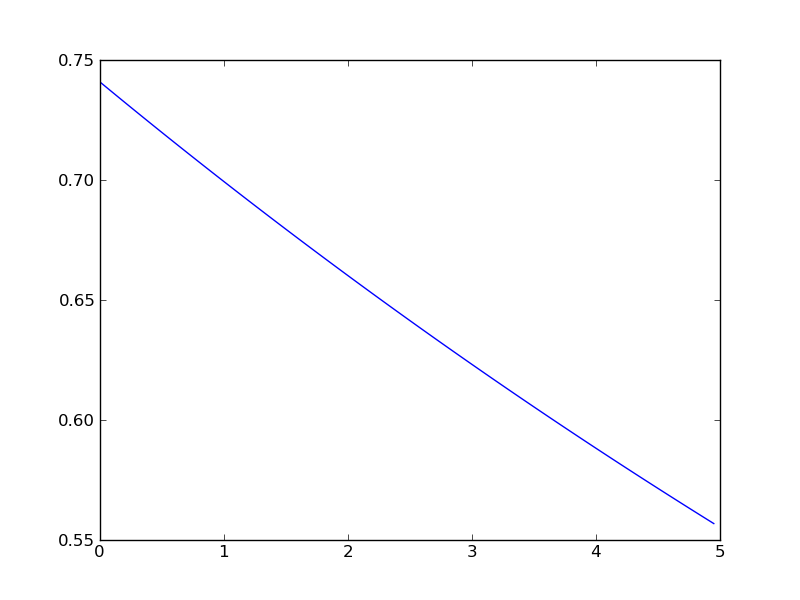
\includegraphics[width=\linewidth]{./images/al/group_0_moment_30}
\caption{Moment $P_5^0$ of the flux for the first group of photons}
\end{minipage}
\hspace{0.5cm}
\begin{minipage}[b]{0.45\linewidth}
\centering
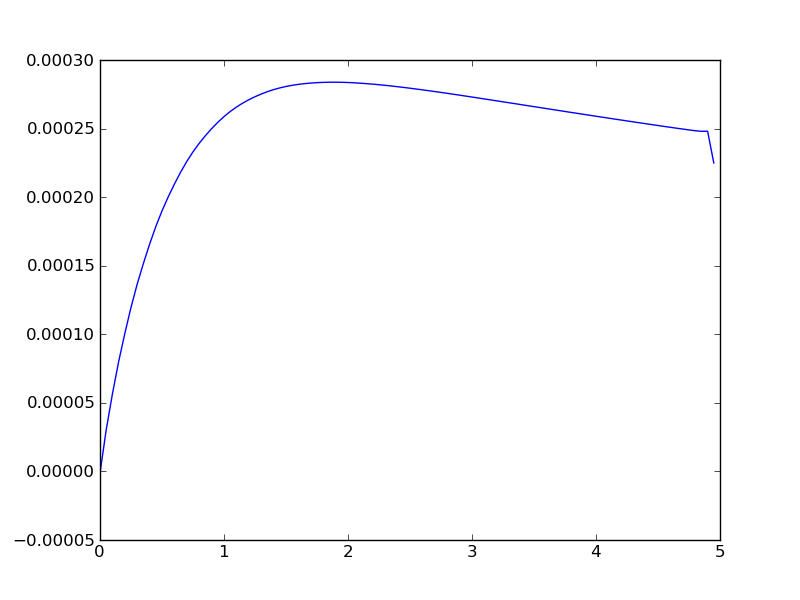
\includegraphics[width=\linewidth]{./images/al/group_39_moment_30}
\caption{Moment $P_5^0$ of the flux for the last group of electrons}
\end{minipage}
\end{figure}

\begin{figure}[H]
\begin{minipage}[b]{0.45\linewidth}
\centering
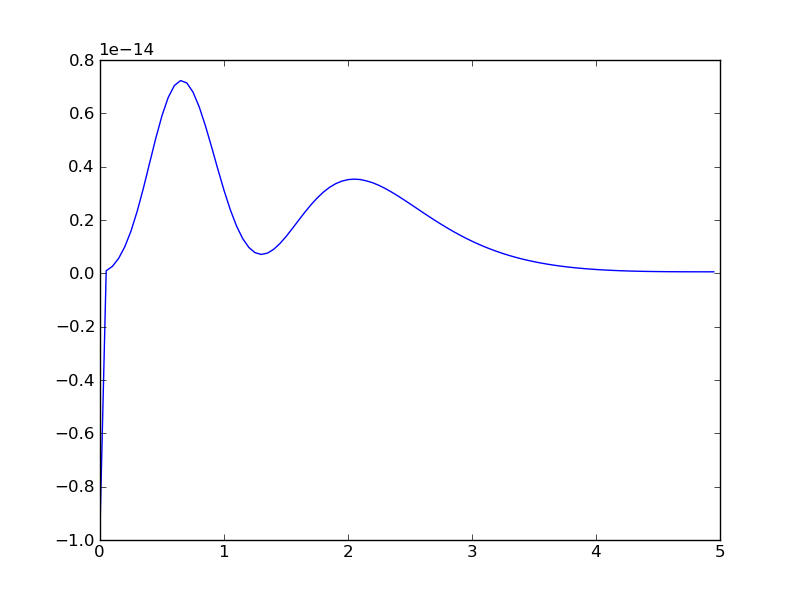
\includegraphics[width=\linewidth]{./images/al/group_0_moment_142}
\caption{Moment $P_{11}^0$ of the flux for the first group of photons}
\end{minipage}
\hspace{0.5cm}
\begin{minipage}[b]{0.45\linewidth}
\centering
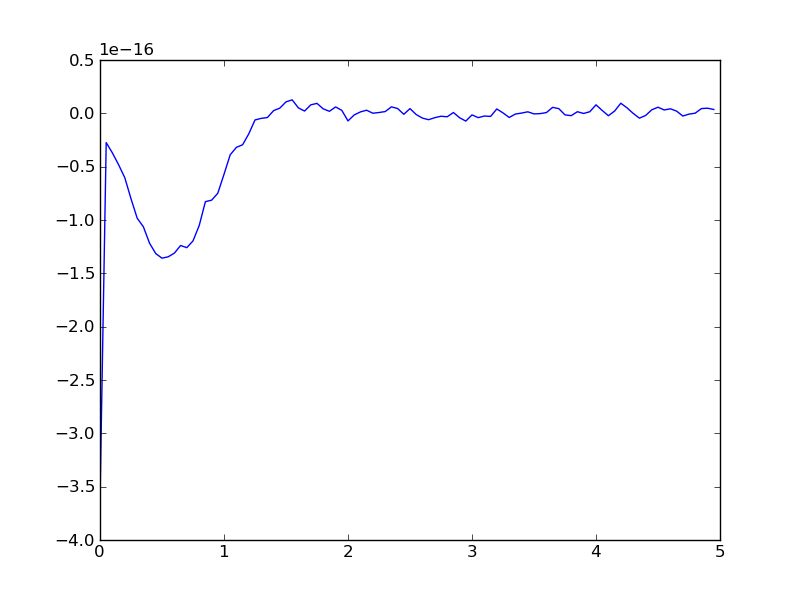
\includegraphics[width=\linewidth]{./images/al/group_39_moment_142}
\caption{Moment $P_5^0$ of the flux for the last group of electrons}
\end{minipage}
\end{figure}

\subsection{Gold}
The setup of this problem is the same as that of the same the others but now 
the medium is made of gold. In the next table, 
we show the dose computed every centimeter using a different scattering order :
\begin{table}[H]
\begin{center}
\caption{Dose in $\frac{MeV}{g}$ for different scattering orders}
\begin{tabular}{|c|c|c|c|c|c|c|}
\hline
Position & ONELDANT & order = 13 & order = 11 & order = 9 & order = 7 & order = 5 \\
\hline
0 & 0.11675 &  &  & 0.097155 & 0.097073 & 0.097326 \\
1 & 0.41799 &  &  & 0.420871 & 0.420988 & 0.421102 \\
2 & 0.16284 &  &  & 0.164946 & 0.165017 & 0.164605 \\
3 & 0.06407 &  &  & 0.065300 & 0.065292 & 0.065214 \\
4 & 0.02566 &  &  & 0.026304 & 0.026295 & 0.026318 \\
5 & 0.00847 &  &  & 0.006083 & 0.006075 & 0.006112 \\
\hline
\end{tabular}
\end{center}
\end{table}     


% Reordering
\section{Reordering}
Another method to decrease memory needed to solve the transport of
electron reorders the energy groups. When CEPXS creates the cross sections,
it first puts in all the cross sections for one particle and then the cross
section for the other particle into the scattering matrix. The cross section 
matrix looks like :
\begin{equation}
S = 
\begin{pmatrix}
A & B\\
C & D
\end{pmatrix}
\end{equation}
where $A$ and $B$ are lower triangular matrices which represents the
scattering for each particle. For each particle, only down scattering
is allowed because the cut-off energy forbids the thermalization of 
particles. The matrices $B$ and $C$ represent the creation of electrons by
photons through photo-electric effect and the creation of photons by
electrons through bremsstrahlung. Now it is important to notice that a
particle can only create a particle which has a energy lower than its own
energy. Moreover, CEPXS forces the maximum energy and the cut-off energy to
be the same for the two particles. For example, theres are two groups for the
photons and four groups for the electrons. The transfer between the groups will 
look \hbox{like :}
\begin{figure}[H]
\begin{center}
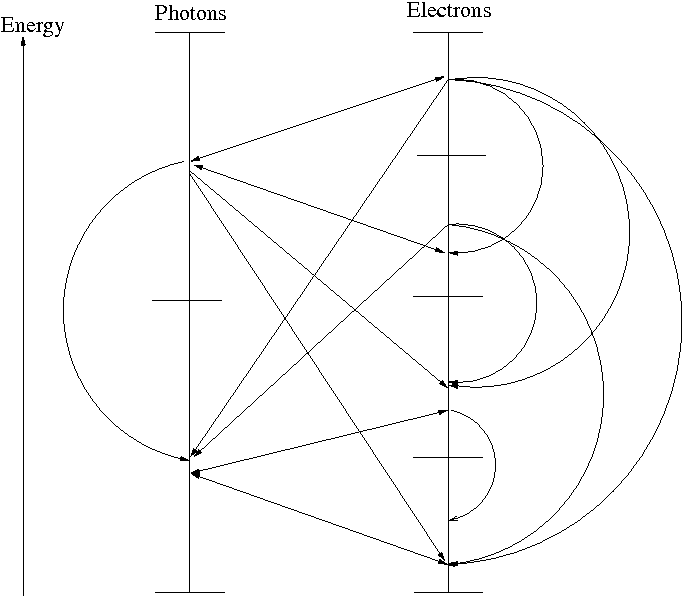
\includegraphics[height=7cm]{group.png}
\caption{Transfer between the different groups}
\end{center}
\end{figure}
The pattern of the scattering matrix looks like :
\begin{equation}
S =
\begin{pmatrix}
x & 0 & x & x & 0 & 0\\
x & x & x & x & x & x\\
x & 0 & x & 0 & 0 & 0\\
x & 0 & x & x & 0 & 0\\
x & x & x & x & x & 0\\
x & x & x & x & x & x\\
\end{pmatrix}
\end{equation}
We can see that there is no upscattering to the first group of photons, the
first and the second group of electrons coming from the second group of
photons and the third or the fourth group of electrons. Thus, if we reorder the 
groups using the following order : photon group 1, electron group 1, electron 
group 2, photon group 2, electron group 3, electron group 4. The pattern of the 
scattering matrix will look like :
\begin{equation}
S =
\begin{pmatrix}
x & x & x & 0 & 0 & 0\\
x & x & 0 & 0 & 0 & 0\\
x & x & x & 0 & 0 & 0\\
x & x & x & x & x & x\\
x & x & x & x & x & 0\\
x & x & x & x & x & x\\
\end{pmatrix}
\end{equation}
Now, we see that we can solve our problem by solving two problems with only three
groups each. We say that we have two group sets of three groups each. We can solve 
the first three groups without solving of the last three groups since there is no 
upscattering coming from these. Then, we can solve the last three groups, with 
the first three groups hidden in the source term. Thus, we can solve a problem
with six groups using the same memory that we would use for only three groups. To 
know how many groups we need to gather from each particle in each group set, we 
can use a simple rule. First, we define the number of groups of photons as
$n_p$, the number of groups electrons as $n_e$ and the greatest common divisor
between these two numbers as $gcd$. The number of groups of photons to put in
a group set is $\frac{n_p}{gcd}$ and the number of groups of electrons to put
in a group set is $\frac{n_e}{gcd}$. Instead of solving one problem of $n$ 
groups, we can solve $gcd$ problems of $\frac{n}{gcd}$ groups.




% Conclusions
\section{Conclusions}
In this paper, we have shown that it is not necessary to keep the full order of
the scattering cross sections to keep an accurate answer while solving
photon-electron transport. Truncating the Galerkin quadrature allows us to
decrease significantly the memory need. We also presented a method to
advantageously reorder the energy groups in the scattering matrix. The groups can 
be reorder in such a way that a problem with $n_p$ groups of photons and $n_e$ 
groups of electrons can be rewritten as $gcd$ problems of $\frac{n_p+n_e}{gcd}$ 
groups, where $gcd$ is the greatest common divisor between $n_p$ and $n_e$. 
These two methods combined allow to decrease significantly the memory needed to 
solve electron transport.


\bibliographystyle{unsrt}
\bibliography{biblio}

\end{document}
